\documentclass[11pt,a4paper]{article}

\usepackage[utf8]{inputenc}
\usepackage[T1]{fontenc}
\usepackage[spanish,es-nodecimaldot]{babel}
\usepackage{mathpazo}
\usepackage{microtype}
\usepackage{geometry}
\geometry{top=1.7cm,bottom=1.8cm,left=2.1cm,right=2.1cm}
\usepackage{graphicx}
\usepackage{xcolor}
\usepackage{booktabs}
\usepackage{array}
\usepackage{enumitem}
\usepackage{hyperref}
\usepackage{caption}
\definecolor{cjcblue}{HTML}{17365D}
\definecolor{cjcgray}{HTML}{5C6670}
\hypersetup{colorlinks=true,urlcolor=cjcblue}
\setlength{\parindent}{0pt}
\setlength{\parskip}{0.57em}
\setlist[itemize]{leftmargin=1.25em,itemsep=0.25em,topsep=0.2em}
\captionsetup{font=footnotesize,labelfont=bf}

\begin{document}
\thispagestyle{empty}


\includegraphics[width=0.43\textwidth]{Paper/figures/logo_cjc_palatino_horizontal.png}
\vspace{0.35cm}

{\color{cjcblue}\rule{\textwidth}{1.1pt}}
\vspace{0.25cm}

{\large\bfseries\color{cjcblue}Comunicado de prensa\par}
\vspace{0.25cm}
{\fontsize{21}{25}\selectfont\bfseries
La PTF del total de la economía cayó 1,5\% entre 2005 y 2024\par}

\vspace{0.35cm}
\begin{itemize}
  \item \textbf{El índice encadenado de la PTF pasó de 100 en 2005 a 98,5 en 2024.}
  \item \textbf{Cuatro actividades aportaron 0,361 puntos porcentuales por año a la PTF total; las otras cinco restaron 0,441 puntos.}
  \item \textbf{Servicios sociales registró la mayor contribución positiva, con 0,148 puntos por año. Finanzas e inmobiliarias tuvo la mayor contribución negativa, con $-0,137$.}
  \item \textbf{La PTF total mejoró después de 2010, pero no inició una trayectoria sostenida de crecimiento.}
\end{itemize}

{\small Bogotá, julio de 2026.}

\textbf{La PTF del total de la economía disminuyó 1,5\% entre 2005 y 2024.}
El nuevo informe del Centro Javeriano de Competitividad (CJC) encadena las 19
variaciones anuales publicadas por el DANE y descompone el resultado entre
nueve actividades económicas. La variación de la PTF total fue, en promedio, de $-0,081$
puntos porcentuales por año.

\textbf{El resultado agregado fue la diferencia entre contribuciones positivas
y negativas de mayor magnitud.} Servicios sociales aportó 0,148 puntos por
año; comercio, 0,128; y agricultura, 0,076. Finanzas e inmobiliarias restó
0,137 puntos; minería, 0,133; y construcción y manufactura, cerca de 0,081 cada
una.

\newpage
\centering
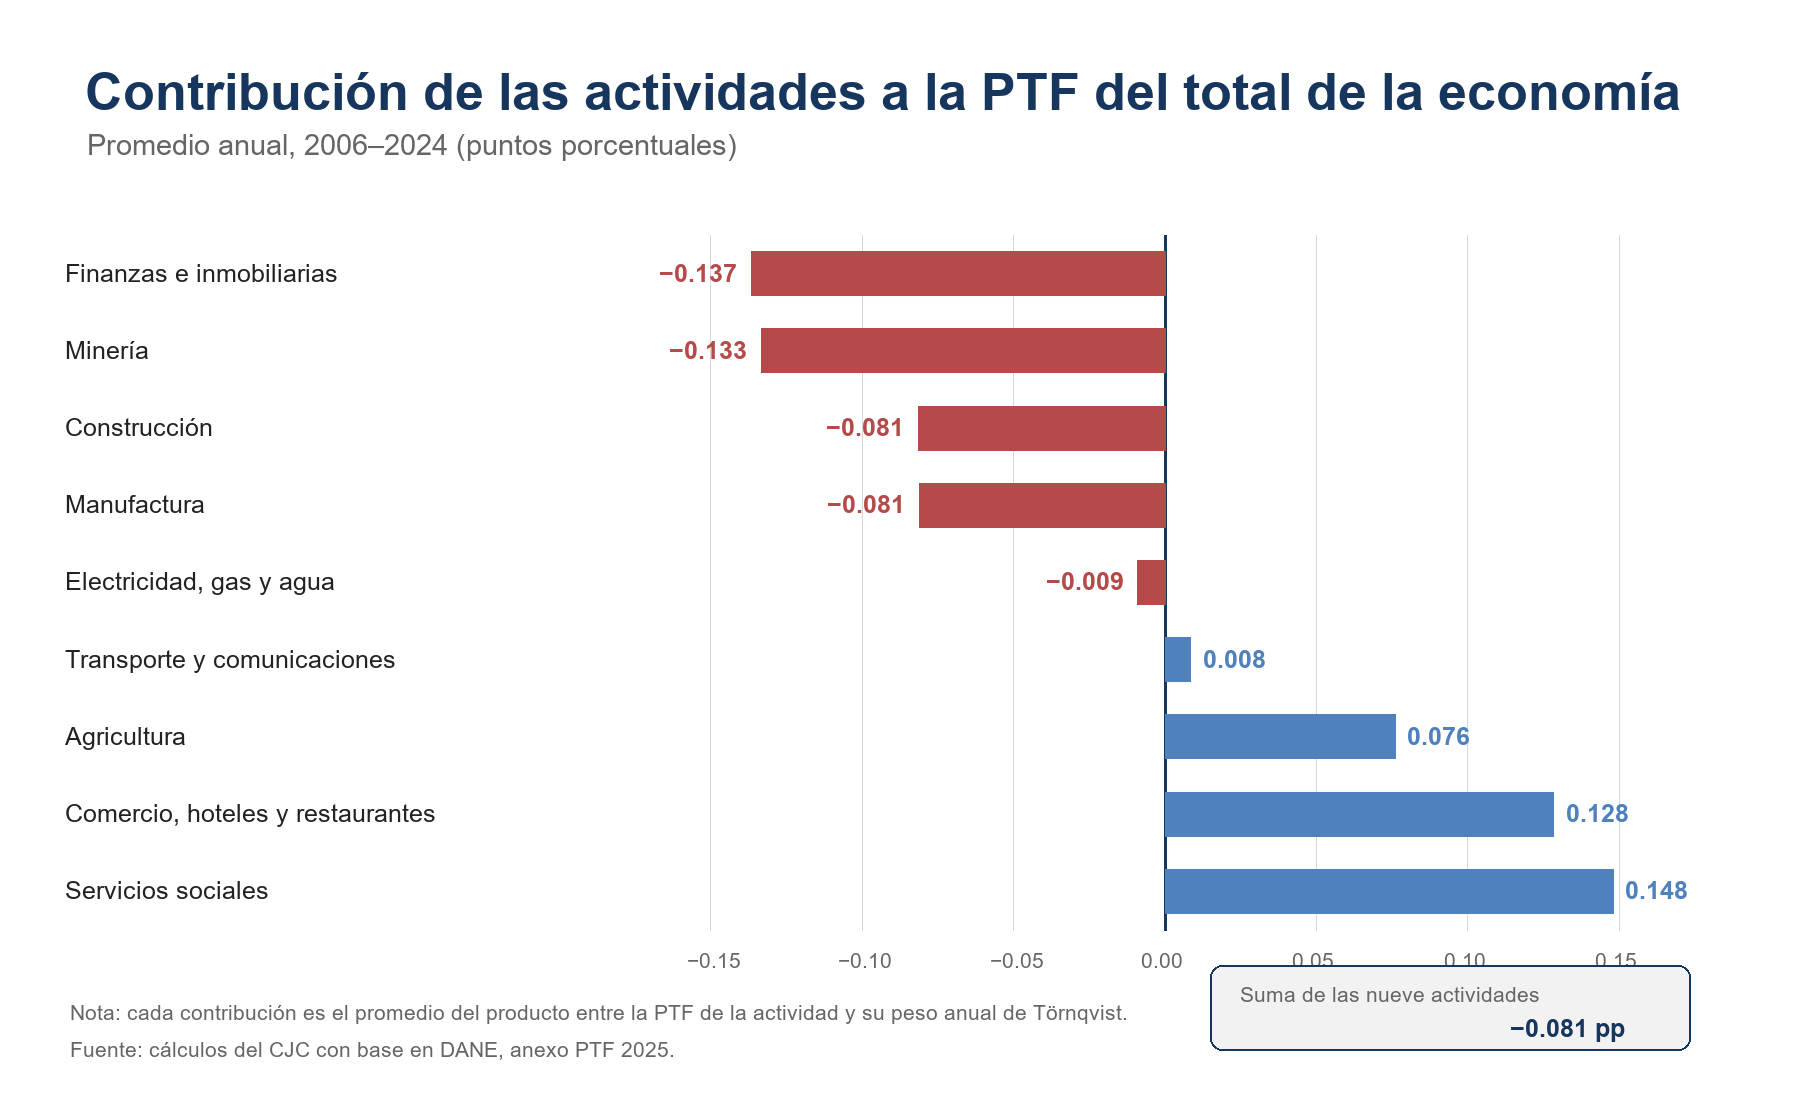
\includegraphics[width=0.91\textwidth]{Paper/figures/fig_ptf_contribucion_total_actividad.png}

{\footnotesize\textit{Fuente:} cálculos del CJC con base en DANE, anexo PTF 2025.\par}
\raggedright

\textbf{La contribución de una actividad depende de su PTF y de su peso en el
valor agregado.} Minería tuvo la mayor caída de la PTF de la actividad, pero
manufactura, con una caída más moderada, tuvo un efecto agregado importante
por su mayor tamaño. Las contribuciones se calculan con las ponderaciones
anuales de Törnqvist que reproducen la PTF total publicada por el DANE.

``La PTF total cercana a cero no significa que todas las actividades se
estancaron. Los aportes de servicios sociales, comercio y agricultura fueron
contrarrestados por las contribuciones negativas de finanzas e inmobiliarias,
minería, construcción y manufactura'', señaló Oliver Pardo, director del
Centro Javeriano de Competitividad.

El análisis usa las 19 variaciones anuales de 2006 a 2024 que enlazan los
niveles de 2005 y 2024. El informe emplea el enfoque de producción, que incluye
trabajo, capital, energía, materiales y servicios. La PTF es el residuo del
crecimiento que no explican esos factores y no debe leerse como una medida pura
de innovación o tecnología.

\textbf{La PTF total mejoró después de 2010, pero permaneció alrededor de
cero.} El promedio fue de $-0,296$ puntos por año en 2006--2010, 0,022 en
2011--2015, $-0,040$ en 2016--2019 y $-0,001$ en 2020--2024. En el último
subperiodo, servicios sociales aportó 0,276 puntos por año, mientras
construcción restó 0,202.

\vfill
{\color{cjcblue}\rule{\textwidth}{0.8pt}}
{\footnotesize
\textbf{Informe completo y materiales reproducibles:}
\href{https://github.com/oliverpardo1979/informe_ptf}{github.com/oliverpardo1979/informe\_ptf}\\
\textbf{Contacto de prensa:} Centro Javeriano de Competitividad,
\href{mailto:competitividad@javeriana.edu.co}{competitividad@javeriana.edu.co}
}

\end{document}
